\documentclass[12pt,a4paper]{article}

\usepackage[T1]{fontenc}
\usepackage[utf8]{inputenc}
\usepackage{lmodern}
\usepackage{microtype}
\usepackage[a4paper,margin=2.54cm]{geometry}
\usepackage{amsmath,amssymb}
\usepackage{graphicx}
\usepackage{array}
\usepackage{xcolor}
\usepackage{caption}
\usepackage{booktabs}
\usepackage{setspace}
\usepackage[mathlines]{lineno}
\usepackage[hidelinks]{hyperref}
\usepackage{subcaption}
\usepackage{tikz}
\usetikzlibrary{positioning,arrows.meta}

\captionsetup{
    font=small,
    labelfont=bf,
    labelsep=period
}
\captionsetup[table]{skip=10pt,position=top}

\setlength{\parindent}{1.5em}
\setlength{\parskip}{0pt}
\setlength{\emergencystretch}{2em}
% Line numbering is available for a later review version but is currently off.
% \modulolinenumbers[5]

\graphicspath{{./}{figures/}}
\newcolumntype{P}[1]{>{\raggedright\arraybackslash}p{#1}}

\usepackage[
backend=biber,
style=numeric,
sorting=none,
giveninits=true,
doi=true,
url=false,
isbn=false
]{biblatex}

\addbibresource{references_agglomerate_gnn.bib}

\begin{document}

\begin{center}
    {\Large\bfseries
    Graph-Based Compression of DEM-Resolved Agglomerate Morphology:\par
    A Preliminary Proof-of-Concept Study\par}
    \vspace{1.25em}
    {\normalsize Ali Khalifa and Heiko Briesen\par}
    \vspace{0.6em}
    {\small Chair of Process Systems Engineering, TUM School of Life Sciences,\par
    Technical University of Munich, Freising, Germany\par}
\end{center}

\vspace{1.25em}
\setstretch{1.5}

\begin{abstract}
	The internal morphology of particle agglomerates can affect shielding and
	accessibility beyond conventional properties such as particle number, size and
	nominal fractal dimension. In this preliminary study, 135 synthetic
	monodisperse agglomerates were generated using a tunable
	particle--cluster/cluster--cluster method that enforces a prescribed
	mass--radius relation. The structures were relaxed using the discrete-element
	method (DEM) to test whether they remained stable under the selected particle
	and contact conditions. The resulting structures were converted into contact
	graphs and characterized using three graph-based shielding proxies: mean graph
	depth, shielded-particle fraction and accessibility score.
	
	A geometry-aware graph neural network was evaluated using grouped five-fold
	cross-validation. The pooled graph representation was compressed into a
	latent bottleneck, and only this latent vector was supplied to the prediction
	head. A one-dimensional latent representation explained approximately $87\,\%$,
	$89\,\%$ and $91\,\%$ of the variability in mean graph
	depth, shielded-particle fraction and accessibility score, respectively. These
	results demonstrate the feasibility of the DEM-to-graph-to-GNN workflow,
	although the current targets are geometric proxies rather than physical
	oxygen-transport quantities. The latent coordinate correlated strongly with
	particle number, radius of gyration, contact count and contact density.
	A separate interpretation analysis showed that conventional scalar descriptors
	could reconstruct approximately $99.6\,\%$ of its variation. The latent
	coordinate should therefore be interpreted as a compact
	size--extent--connectivity coordinate rather than an independent geometrical
	descriptor. Particle count alone reached a mean $R^2$ of at most $0.776$ for
	predicting the three targets, compared with $0.892$ for the GNN. Models using
	six conventional size and contact descriptors reached $0.891$ with linear
	regression and $0.909$ with a random forest. Thus, the GNN clearly improved on
	particle count alone and achieved accuracy comparable to the multidescriptor
	models, while compressing the complete graph into a single learned coordinate.
\end{abstract}

\noindent\textbf{Keywords:} particle agglomerates; discrete-element method;
contact graphs; graph neural networks; latent morphology representation;
transport accessibility

% Activate for journal review only when required:
% \linenumbers

\section{Introduction}
\label{sec:introduction}

Transport models for biological and cohesive particle aggregates commonly
describe morphology using a small set of integral quantities, such as aggregate
diameter, porosity or fractal dimension. Such descriptors are useful, but they
do not uniquely determine the internal arrangement of the primary particles.
Aggregates with similar integral properties can still differ in connectivity,
surface exposure, shielding and the existence of internal transport pathways.
These structural differences may subsequently influence substrate or oxygen
accessibility and therefore the effective activity of an aggregate.

The broader research concept is to derive morphology-aware oxygen-transport
closures from particle-resolved CFD--DEM simulations and use them in
coarse-scale CFD--PBM or Euler--Lagrange reactor models. In that future
framework, a graph neural network would encode the detailed particle structure
into a compact morphology descriptor, while a reduced closure would combine
this descriptor with local reactor conditions to predict oxygen uptake, dynamic
response and the fraction of oxygen-limited cells.

Before conducting expensive coupled flow and transport simulations, the present
DEM-only study tests the feasibility of the structural part of this concept.
Its central hypothesis is that a particle-contact graph contains nonlocal
morphological information that can be compressed into a low-dimensional latent
representation without losing the information required to predict internal
shielding. The study therefore addresses three preliminary questions:
\begin{enumerate}
    \item Can generated agglomerates be mechanically relaxed and converted
    consistently into particle-contact graphs?
    \item Can a GNN predict nonlocal shielding and accessibility measures for
    parameter combinations withheld from training?
    \item How many latent variables are required to retain this structural
    information?
\end{enumerate}

The calculated targets are intentionally limited to geometric graph proxies.
This separation is important: the study validates the computational workflow
and the concept of morphology compression, while the physical relation to
oxygen transport remains a task for the proposed particle-resolved project.

The proof-of-concept study proceeds in six steps. First, synthetic
agglomerates are generated with different particle counts and physical sizes,
as well as with equal particle counts but different compactness settings and
random particle arrangements. Second, the artificial structures are relaxed
in a physical DEM environment to test whether they remain mechanically stable
under the selected particle and contact forces. Third, three structural
targets are defined to quantify depth, shielding and accessibility relative to
the outer surface. Fourth, each relaxed agglomerate is converted into a
particle-contact graph. Fifth, a GNN is trained to compress the graph into one
or more latent descriptors while retaining the information needed to predict
the three targets. Finally, the learned descriptor is interpreted by comparing
it with conventional physical and graph-based measures, and its predictive
value is tested against particle count alone and against models using several
conventional descriptors together. The complete workflow is summarized in
Fig.~\ref{fig:study_workflow}.

\begin{figure}[!tbp]
	\centering
	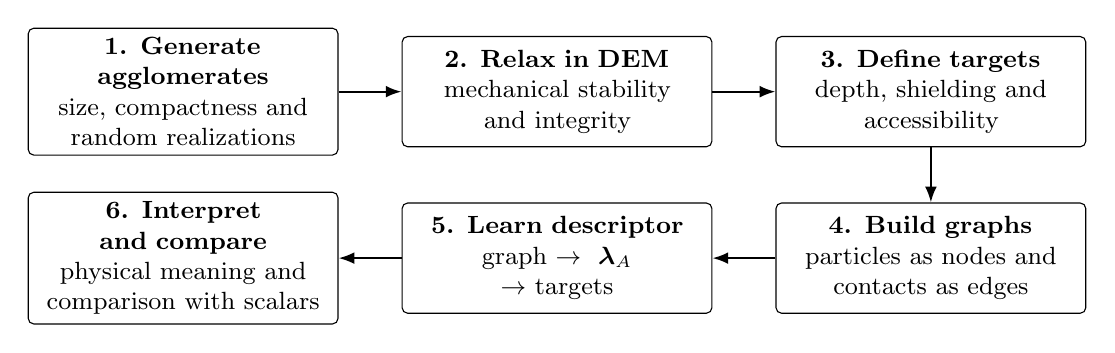
\begin{tikzpicture}[
		node distance=7mm and 8mm,
		workflowbox/.style={
			draw,
			rounded corners=2pt,
			align=center,
			minimum height=14mm,
			text width=3.7cm,
			font=\small
		},
		arrow/.style={-{Latex[length=2mm]}, thick}
	]
		\node[workflowbox] (generation) {
			\textbf{1. Generate agglomerates}\\
			size, compactness and\\random realizations
		};
		\node[workflowbox, right=of generation] (relaxation) {
			\textbf{2. Relax in DEM}\\
			mechanical stability\\and integrity
		};
		\node[workflowbox, right=of relaxation] (targets) {
			\textbf{3. Define targets}\\
			depth, shielding and\\accessibility
		};
		\node[workflowbox, below=of targets] (graphs) {
			\textbf{4. Build graphs}\\
			particles as nodes and\\contacts as edges
		};
		\node[workflowbox, left=of graphs] (compression) {
			\textbf{5. Learn descriptor}\\
			graph $\rightarrow \boldsymbol{\lambda}_A$\\$\rightarrow$ targets
		};
		\node[workflowbox, left=of compression] (interpretation) {
			\textbf{6. Interpret and compare}\\
			physical meaning and\\comparison with scalars
		};

		\draw[arrow] (generation) -- (relaxation);
		\draw[arrow] (relaxation) -- (targets);
		\draw[arrow] (targets) -- (graphs);
		\draw[arrow] (graphs) -- (compression);
		\draw[arrow] (compression) -- (interpretation);
	\end{tikzpicture}
	\caption{Six-step workflow used to generate and relax synthetic
	agglomerates, represent them as graphs, learn a compact structural
	descriptor and evaluate its physical meaning and predictive value.}
	\label{fig:study_workflow}
\end{figure}

\section{Methodology and computational workflow}
\label{sec:preliminary_dem_gnn}

\subsection{Synthetic agglomerate ensemble}

The preliminary data set consists of monodisperse agglomerates generated with
the tunable particle--cluster and cluster--cluster aggregation formulation of
Filippov, Zurita and Rosner~\cite{Filippov2000}, following the efficient
hierarchical implementation described by Skorupski et
al.~\cite{Skorupski2014}. The method prescribes the mass--radius relation
\begin{equation}
    N=k_f\left(\frac{R_g}{r_p}\right)^{D_f},
    \label{eq:fractal_mass_radius}
\end{equation}
where $N$ is the number of primary particles, $r_p$ is their radius, $R_g$ is
the radius of gyration including the finite primary-particle radius, $D_f$ is
the requested fractal dimension and $k_f$ is the fractal prefactor.

Generation begins with stochastic 25-particle seed clusters. Starting from two
touching particles, further particles are placed at random orientations on the
radial shell required by Eq.~\eqref{eq:fractal_mass_radius}; placements are
accepted only when they establish contact without overlap. Equal-sized seed
clusters are subsequently combined hierarchically. Before each merge, both
subclusters are randomly rotated. Their prescribed center-of-mass separation
$R_{12}$ follows from the parallel-axis relation,
\begin{equation}
 R_{12}^{2}=
 r_p^2\frac{N^2}{N_1N_2}
 \left(\frac{N}{k_f}\right)^{2/D_f}
 -\frac{N}{N_2}R_{g,1}^{2}
 -\frac{N}{N_1}R_{g,2}^{2},
 \qquad N=N_1+N_2.
 \label{eq:cca_separation}
\end{equation}
A Monte Carlo orientation search identifies a non-overlapping configuration
whose first-contact separation agrees with $R_{12}$ within the prescribed
tolerance. The clusters are placed at this analytically determined
first-contact distance, guaranteeing connectivity without overlap while
allowing only a small, recorded deviation from the requested mass--radius law.
The particle counts $N=50$, 100 and 200 correspond to one, two and three
hierarchical merging levels, respectively, from the common 25-particle seeds.

Three morphology settings were used: $(D_f,k_f)=(1.8,1.3)$ for open,
$(2.2,1.1)$ for intermediate and $(2.6,0.8)$ for comparatively compact
agglomerates. The word ``compact'' is relative to the other fractal cases: the
cluster--cluster construction creates contact-connected fractal structures and
does not imply dense, nearly spherical packing. Dense spherical clusters would
require an additional restructuring or densification procedure
\cite{Ehrl2009}.

The data set comprises three primary-particle diameters, three particle counts,
three morphology settings and five independent random realizations per design
point,
\begin{equation*}
	3\ \text{diameters}\times3\ \text{particle counts}
	\times3\ \text{morphologies}\times5\ \text{realizations}
	=135\ \text{agglomerates}.
\end{equation*}
The details are summarized in Table~\ref{tab:sim_parameter}.


\begin{table}[!tbp]
	\centering
	\caption{Design variables used in the DEM investigation.}
	\label{tab:sim_parameter}
	\begin{tabular}{p{0.39\linewidth} p{0.51\linewidth}}
		\toprule
		\textbf{Design variable} & \textbf{Values} \\
		\midrule
		Primary-particle diameter $d_p$
		& $1.0$, $1.5$, $2.0\,\mu\mathrm{m}$ \\
		Number of particles $N$
		& $50$, $100$, $200$ \\
		Requested $(D_f,k_f)$ and morphology
		& $(1.8,1.3)$ open; $(2.2,1.1)$ intermediate;
		$(2.6,0.8)$ comparatively compact \\
		Random realizations
		& $5$ per parameter combination \\
		Total number of cases
		& $135$ \\
		\bottomrule
	\end{tabular}
\end{table}

Each realization was assigned a unique random seed. The generated particle
coordinates and radii were exported in formats suitable for DEM relaxation,
graph construction and visualization. All particles represented the same
material; no permanent bonds were prescribed, and the initial translational
and angular velocities were zero.

% Common crop for all three images:
% trim order: left, bottom, right, top

\begin{figure}[!tbp]
	\centering
	
	\begin{subfigure}[t]{0.32\textwidth}
		\centering
		
\includegraphics[
		width=0.75\linewidth,
		trim={450bp 5bp 450bp 5bp},
		clip
		]{open.png}
		\caption{Open aggregate}
		\label{fig:agg_open}
	\end{subfigure}
	\hfill
	\begin{subfigure}[t]{0.32\textwidth}
		\centering
		
\includegraphics[
		width=0.75\linewidth,
		trim={450bp 5bp 450bp 5bp},
		clip
		]{intermediate.png}
		\caption{Intermediate aggregate}
		\label{fig:agg_intermediate}
	\end{subfigure}
	\hfill
	\begin{subfigure}[t]{0.32\textwidth}
		\centering
		
\includegraphics[
		width=0.75\linewidth,
		trim={450bp 5bp 450bp 5bp},
		clip
		]{compact.png}
		\caption{Comparatively compact aggregate}
		\label{fig:agg_compact}
	\end{subfigure}
	
	\caption{Representative post-DEM agglomerates illustrating the range of
		morphologies in the preliminary data set. The three agglomerates have the
		same primary-particle diameter ($d_p=$ 2 $\mu$m) and particle count ($N=$200) but different requested
		$(D_f,k_f)$ morphology settings. The particles are coloured according to
		their graph depth $h_i$, as defined below, using a common colour scale
		ranging from $0$ to $11$.}
	\label{fig:representative_agglomerates}
\end{figure}

\subsection{DEM relaxation and stability assessment}

The generated structures were mechanically relaxed using a soft-sphere DEM
formulation. Normal contact was described by Hertzian elastic repulsion and
regularized van der Waals attraction. The adhesive interaction is governed by
the Hamaker constant $A_H$ and a minimum surface separation $h_{\min}$, which
removes the singularity of the idealized interaction at vanishing separation
\cite{Hamaker1937,Israelachvili2011}. Tangential resistance was evaluated from
the contact history and limited by Coulomb friction. Rolling and torsional
resistance were also included. No permanent bonds were introduced; the relaxed
structures were maintained solely by adhesion and contact friction. The applied contact models are summarized in Table~\ref{tab:dem_contact_model}.
\begin{table}[!tbp]
	\centering
	\caption{Contact formulation used for DEM relaxation.}
	\label{tab:dem_contact_model}
	\begin{tabular}{P{0.32\linewidth} P{0.58\linewidth}}
		\toprule
		\textbf{Model component} &
		\textbf{Physical formulation} \\
		\midrule
		Normal interaction &
		Hertzian elastic repulsion combined with regularized van der Waals
		attraction \\
		
		Tangential interaction &
		History-dependent tangential force with Coulomb limitation \\
		
		Rolling resistance &
		Directional rolling-resistance torque \\
		
		Torsional resistance &
		Resistance to relative twisting at a contact \\
		
		Near-contact regularization &
		Limitation of nonphysical normal-force states near contact \\
		
		Permanent bonds &
		None \\
		\bottomrule
	\end{tabular}
\end{table}

Although the numerical setup permits multiple material types, identical
properties were used for every interaction in the present monodisperse study.
\begin{table}[!tbp]
	\centering
	\caption{Particle and contact parameters used in the DEM relaxation.
		The primary-particle diameter was varied, while the remaining properties
		were held constant.}
	\label{tab:dem_material_parameters}
	\begin{tabular}{p{0.39\linewidth} p{0.16\linewidth} p{0.29\linewidth}}
		\toprule
		\textbf{Property} & \textbf{Symbol} & \textbf{Value} \\
		\midrule
		Particle shape
		& -- & Sphere \\
		Primary-particle diameter
		& $d_p$ & $1.0$, $1.5$, $2.0\,\mu\mathrm{m}$ \\
		Reference particle density
		& $\rho_p$ & $1050\,\mathrm{kg\,m^{-3}}$ \\
		Young's modulus
		& $E$ & $1.0\times10^{9}\,\mathrm{Pa}$ \\
		Poisson ratio
		& $\nu$ & $0.45$ \\
		Coefficient of restitution
		& $e$ & $0.20$ \\
		Sliding-friction coefficient
		& $\mu$ & $0.30$ \\
		Rolling-friction coefficient
		& $\mu_r$ & $0.01$ \\
		Hamaker constant
		& $A_H$ & $3.028\times10^{-20}\,\mathrm{J}$ \\
		Minimum separation distance
		& $h_{\min}$ & $4.0\times10^{-10}\,\mathrm{m}$ \\
		\bottomrule
	\end{tabular}
\end{table}

The primary-particle diameters of $1.0$--$2.0\,\mu\mathrm{m}$ represent the
characteristic micrometre scale of many bacterial cells
\cite{LevinAngert2015}. The range is intentionally narrow:
its purpose in this preliminary study is to test whether the graph workflow
remains consistent when the physical length scale changes, while particle
number and morphology are varied independently. The density
$\rho_p=1050\,\mathrm{kg\,m^{-3}}$ represents a water-rich particle only
slightly denser than the surrounding liquid. Measurements for
\textit{Escherichia coli}, for example, place the buoyant density near
$1080$--$1105\,\mathrm{kg\,m^{-3}}$ \cite{MartinezSalas1981,Woldringh1981}.
The slightly lower reference value used here is therefore an idealized
near-neutral-buoyancy choice rather than a species-specific measurement. The
Poisson ratio $\nu=0.45$ represents a nearly incompressible effective particle.

The remaining mechanical parameters define a controlled relaxation model and
must not be interpreted as a calibrated constitutive description of a
particular microorganism. Reported effective bacterial-envelope moduli are
commonly in the MPa range and depend strongly on species, physiological state
and measurement protocol \cite{Deng2011,Lee2024}; the present value
$E=1\,\mathrm{GPa}$ was selected as a stiff numerical contact parameter to
restrict overlap during relaxation. The low restitution coefficient provides
strong damping, whereas the sliding- and rolling-friction coefficients resist
relative translation and rotation. The adopted Hamaker constant is of the
conventional $10^{-20}\,\mathrm{J}$ order associated with dispersion
interactions, but its effective value depends on the interacting materials and
the intervening liquid \cite{Israelachvili2011}. Accordingly, elasticity,
dissipation, friction and adhesion should be varied in a sensitivity study and
calibrated before applying the model to a specific bioaggregate. The relevant particle and contact parameters used in the present DEM relaxation simulations are listed in Table~\ref{tab:dem_material_parameters}.

%The particle density is inherited from the particle initialization data. Its
%value should therefore be verified directly in these files before the present
%study is submitted for publication.
%
%For the specified Hamaker constant and minimum separation, the corresponding
%planar work-of-adhesion estimate is
%\begin{equation}
% W=\frac{A_H}{12\pi h_{\min}^{2}}
%   \approx 5.0\times10^{-3}\,\mathrm{J\,m^{-2}}.
%\end{equation}
%This value characterizes the effective adhesion used in the preliminary
%relaxation and is not presented as a universally valid biological material
%constant.
The relaxation simulations were performed with a physical time step of
$\Delta t=5.0\times10^{-11}\,\mathrm{s}$ and were run for up to $300000$ time
steps, corresponding to a maximum physical duration of
$1.5\times10^{-5}\,\mathrm{s}=15\,\mu\mathrm{s}$. The purpose of this DEM stage
was to obtain mechanically stable structures and to verify that the
artificially generated agglomerates remained intact under the selected
elasticity, dissipation, friction and adhesive-contact conditions without
permanent bonds. The suitability of the time step was checked every $1000$
steps against the characteristic contact and neighbour-list time scales.
Particle and pair-interaction data were written every $20000$ steps,
corresponding to output intervals of $1\,\mu\mathrm{s}$. Gravity was not
activated because the simulation focused on internal contact-scale relaxation
without sedimentation or an externally imposed loading direction.

The particle output contained positions, radii, particle IDs and velocities,
whereas the pair output contained interacting particle IDs, gap, overlap,
contact area, normal and tangential forces, total force and torque. These data
were converted to VTK for inspection and subsequent graph construction.
Because the adhesive interaction also acts across a finite gap, a reported
particle pair does not necessarily represent a geometrically touching contact.
The pairs were therefore classified using
\begin{equation}
	\delta_{ij}
	=r_i+r_j-\lVert\boldsymbol{x}_i-\boldsymbol{x}_j\rVert .
\end{equation}
Pairs satisfying
$\delta_{ij}/d_{\mathrm{ref}}\geq-10^{-6}$ were treated as touching. This small
tolerance retains numerically near-touching pairs while excluding separated
neighbours interacting only through finite-range adhesive forces.

For each case, particle and contact VTK files were matched by time step. An
agglomerate was considered relaxed when, over three consecutive output
intervals,
\begin{equation}
	\frac{\Delta x_{\mathrm{RMS}}}{d_p}\leq10^{-4},
	\qquad
	1-\frac{|C_k\cap C_{k+1}|}{|C_k\cup C_{k+1}|}\leq0.01,
\end{equation}
where $C_k$ denotes the set of particle contacts at time step $k$. These
criteria require both the particle positions and the contact network to become
nearly stationary.

Agglomerate integrity was evaluated independently using connected-component
analysis. Each particle was treated as a graph node and every reported
particle-pair interaction as an undirected edge. All 135 final structures
contained exactly one connected component with a largest-component fraction of
unity. Thus, none of the artificially generated agglomerates fragmented during
the DEM relaxation.

\subsection{Effective fractal-dimension characterization}
\label{sec:measured_fractal_dimension}

The fractal dimensions specified during agglomerate generation define the
requested morphology settings. Since the generated structures contain only
\(50\)--\(200\) primary particles and are subsequently relaxed by DEM, these
input values should not be interpreted as exact measured properties of every
final structure. The relaxed agglomerates were therefore characterized using
two complementary finite-scale methods. Both methods are commonly used to
characterize particle aggregates, although their estimates can depend on the
available scale range and the finite number of primary particles
\cite{Bushell2002,Theiler1990}.

The first estimate was based on the mass--radius scaling relation commonly
used for fractal particle aggregates \cite{Sorensen2001,Bushell2002},
\begin{equation}
	N(r)\propto r^{D_f},
\end{equation}
where \(N(r)\) is the number of particle centres within a distance \(r\) from
the agglomerate centre of mass. After calculating the distance of every
particle centre from the agglomerate centre of mass, the particles were sorted
according to this radial distance. The effective fractal dimension was then
obtained from the slope of
\begin{equation}
	\log N(r)=D_f\log r+C.
\end{equation}
Only the range containing \(10\)--\(80\,\%\) of the particles was included in
the regression. The innermost region was excluded because it contains only a
small number of particles, while the outermost region is strongly affected by
the finite boundary of the agglomerate.

A second estimate was obtained using the box-counting method
\cite{Liebovitch1989,ForoutanPour1999,Theiler1990}. The particle centres were
covered by a three-dimensional Cartesian grid with box size \(\epsilon\), and
the number of boxes containing at least one particle centre,
\(N_{\mathrm{box}}(\epsilon)\), was counted. The effective box-counting
dimension follows from
\begin{equation}
	N_{\mathrm{box}}(\epsilon)
	\propto \epsilon^{-D_f},
\end{equation}
and was calculated as the slope of
\(\log N_{\mathrm{box}}\) against \(\log(1/\epsilon)\).

Before box counting, each agglomerate was translated to its centre and aligned
with its principal axes. Twelve logarithmically spaced box sizes were
evaluated. For each box size, 32 shifted grids were tested and the smallest
occupied-box count was retained to reduce sensitivity to the arbitrary grid
origin. Scales for which nearly all particles occupied separate boxes, as well
as scales for which the complete agglomerate occupied approximately one box,
were excluded. Such scale selection is important because both limits contain
little information about the intermediate spatial scaling
\cite{ForoutanPour1999,Theiler1990}.

\subsection{Graph representation and structural targets}

Each selected agglomerate snapshot was represented as a contact graph. Primary particles
form the nodes, while only geometrically touching or numerically near-touching
pairs satisfying $\delta_{ij}/d_{\mathrm{ref}}\geq-10^{-6}$ form the edges.
Separated attractive neighbours were excluded. This choice gives the graph a
clear geometrical interpretation and prevents its topology from depending on
the finite interaction cutoff of the adhesive model. Every retained pair was
stored in both directions for message passing. Thus, an agglomerate with $N$
particles and $N_c$ retained contacts has $N$ nodes and $2N_c$ directed edges.
All 135 agglomerates yielded valid graphs and were included in the analysis;
no case was skipped.

Three node features were available after preprocessing. The minimal model used
the two nonconstant structural scalars
\begin{equation}
 \boldsymbol{x}_i=
 \left[
   \frac{|\boldsymbol{x}_i-\boldsymbol{x}_c|}{R_g},\;
   z_i
 \right],
\end{equation}
where $d_{\mathrm{ref}}$ is twice the median particle radius,
$\boldsymbol{x}_c$ is the agglomerate center, $R_g$ is the radius of gyration,
and $z_i$ is the coordination number. The third available node feature,
$r_i/d_{\mathrm{ref}}$, is approximately $0.5$ for all present monodisperse
particles and was therefore omitted from the minimal model.

The processed DEM data contained 22 available contact features, including
normalized distance and overlap, gap, contact area, force and torque quantities
and contact-state flags. For the minimal model, only the normalized centre
distance $d_{ij}/d_{\mathrm{ref}}$ was selected from these stored contact
features, because connectivity and interparticle geometry are the quantities
directly relevant to the three structural targets considered here. The graph
connectivity and normalized relative-position vector were additionally used
for message passing. The remaining available contact features were retained
for possible sensitivity studies but were not supplied to the reported model.

The convex hull of the particle centres was calculated using the Qhull option
\texttt{QJ}. Particles located at the hull vertices were classified as surface
particles and assigned a graph depth of \(h_i=0\). The graph depth of every
other particle was defined as the minimum number of contact connections
required to reach a surface particle.

Three aggregate-level quantities were then calculated:
\begin{align}
	\overline{h} &= \frac{1}{N}\sum_{i=1}^{N}h_i,\\
	f_{h\geq2} &= \frac{1}{N}\sum_{i=1}^{N}\mathbf{1}(h_i\geq2),\\
	S_{\mathrm{access}} &= \frac{1}{N}\sum_{i=1}^{N}\exp(-\beta h_i),
	\qquad \beta=0.5.
\end{align}

The mean graph depth \(\overline{h}\) indicates how deeply the particles are
located within the aggregate. A larger value represents a more strongly
shielded internal structure. The quantity \(f_{h\geq2}\) is the fraction of
particles that are separated from the surface by at least two contact
connections and therefore represents the strongly shielded particle fraction.
Finally, \(S_{\mathrm{access}}\) is a continuous accessibility score: surface
particles contribute \(1\), while the contribution of internal particles
decreases exponentially with graph depth. Consequently, values closer to one
indicate a more accessible aggregate, whereas lower values indicate stronger
internal shielding.

These quantities are deliberately defined geometric proxies derived from the
contact network. They test whether a GNN can distinguish aggregate structures
with different degrees of internal shielding; they do not yet represent oxygen
transport or oxygen uptake.

\subsection{GNN compression and training}

In addition to the stored node and edge features, the model uses the particle
coordinates relative to the aggregate centre and normalized by the reference
diameter $d_{\mathrm{ref}}$. The corresponding relative-position vector is
assigned to every directed edge. Random rigid rotations are applied during
training to prevent the model from associating the target quantities with a
particular aggregate orientation.

The node and edge inputs are embedded into a hidden space of dimension 64.
Six residual GINE message-passing layers with layer normalization and dropout
are then applied. The message-passing depth allows information to propagate
over extended paths through the aggregate, while the residual connections
reduce optimization difficulties and the loss of local information. Graph-level
mean, maximum and size-sensitive normalized-sum pooling are combined to form a
graph-derived aggregate representation. This representation alone is
compressed through the latent bottleneck into a morphology vector
\begin{equation}
	\boldsymbol{\lambda}_A =
	\left[\lambda_1,\ldots,\lambda_{n_\lambda}\right]
	\in \mathbb{R}^{n_\lambda},
\end{equation}
where the latent dimension $n_\lambda$ is treated as a model hyperparameter.
Candidate values $n_\lambda\in\{1,2,3,4\}$ are evaluated by grouped
cross-validation. Thus, the GNN learns the values of the latent components,
whereas their required number is determined from the predictive performance
and model-complexity comparison.

No separately calculated aggregate-level descriptors are supplied to either
the latent bottleneck or the prediction head. Aggregate size, spatial extent
and connectivity can nevertheless be inferred from the number and arrangement
of nodes, their normalized coordinates, the contact topology and the
size-sensitive normalized-sum pooling term. A two-layer prediction head maps
only $\boldsymbol{\lambda}_A$ to the three supervised proxy targets,
\begin{equation}
	\widehat{\boldsymbol{y}}_A =
	\left[
	\widehat{\overline{h}},\;
	\widehat{f}_{h\geq2},\;
	\widehat{S}_{\mathrm{access}}
	\right].
\end{equation}

Training used Adam with a learning rate of $10^{-3}$, weight decay of $10^{-5}$,
batch size 16 and random seed 7. The targets were standardized using only the
respective training data. A validation subset and early stopping were used to
retain the best model in each fold instead of automatically selecting the last
training epoch.


% In the document
\begin{figure}[!tbp]
	\centering
	\resizebox{0.99\textwidth}{!}{%
	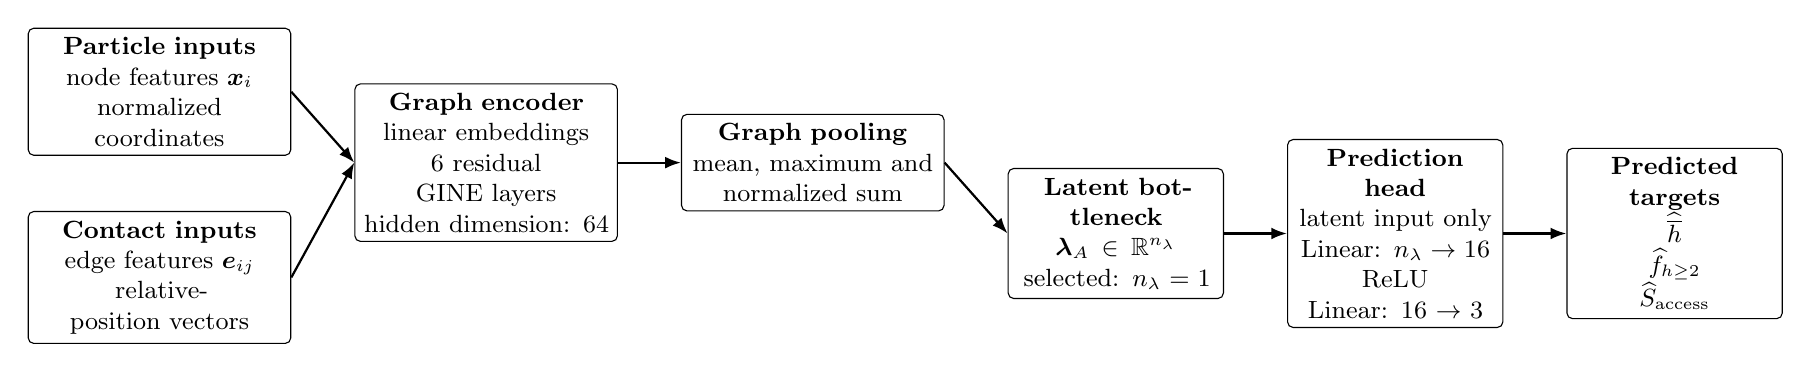
\begin{tikzpicture}[
		node distance=7mm and 8mm,
		block/.style={
			draw,
			rounded corners=2pt,
			align=center,
			minimum height=11mm,
			text width=3.1cm,
			font=\small
		},
		smallblock/.style={
			draw,
			rounded corners=2pt,
			align=center,
			minimum height=10mm,
			text width=2.5cm,
			font=\small
		},
		arrow/.style={-{Latex[length=2mm]}, thick}
		]
		
		% Graph-level inputs
		\node[block] (nodeinput) {
			\textbf{Particle inputs}\\
			node features $\boldsymbol{x}_i$\\
			normalized coordinates
		};
		
		\node[block, below=of nodeinput] (edgeinput) {
			\textbf{Contact inputs}\\
			edge features $\boldsymbol{e}_{ij}$\\
			relative-position vectors
		};
		
		% GNN
		\node[block, right=of nodeinput, yshift=-9mm] (gine) {
			\textbf{Graph encoder}\\
			linear embeddings\\
			$6$ residual GINE layers\\
			hidden dimension: $64$
		};
		
		% Pooling
		\node[block, right=of gine] (pooling) {
			\textbf{Graph pooling}\\
			mean, maximum and\\
			normalized sum
		};
		
		% Latent representation
		\node[smallblock, right=of pooling, yshift=-9mm] (latent) {
			\textbf{Latent bottleneck}\\
			$\boldsymbol{\lambda}_A
			\in\mathbb{R}^{n_\lambda}$\\
			selected: $n_\lambda=1$
		};
		
		% Prediction head
		\node[smallblock, right=of latent] (head) {
			\textbf{Prediction head}\\
			latent input only\\
			Linear: $n_\lambda\rightarrow16$\\
			ReLU\\
			Linear: $16\rightarrow3$
		};
		
		% Outputs
		\node[smallblock, right=of head] (output) {
			\textbf{Predicted targets}\\
			$\widehat{\overline h}$\\
			$\widehat f_{h\geq2}$\\
			$\widehat S_{\mathrm{access}}$
		};
		
		% Arrows
		\draw[arrow] (nodeinput.east) -- (gine.west);
		\draw[arrow] (edgeinput.east) -- (gine.west);
		\draw[arrow] (gine.east) -- (pooling.west);
		\draw[arrow] (pooling.east) -- (latent.west);
		\draw[arrow] (latent.east) -- (head.west);
		\draw[arrow] (head.east) -- (output.west);
		
	\end{tikzpicture}}
	
	\caption{Architecture of the graph-based morphology model. Particle and
		contact information is processed by the message-passing graph encoder.
		The pooled graph representation is compressed into the latent morphology
		vector $\boldsymbol{\lambda}_A$. A two-layer multilayer perceptron maps only
		this latent vector to the three supervised geometric targets. All
		components are trained jointly.}
	\label{fig:gnn_architecture}
\end{figure}

The assessment used grouped five-fold cross-validation. All five random
realizations with the same $(d_p,N,D_f,k_f)$ combination were assigned to the
same test fold. This produced 27 parameter groups.
Consequently, each reported prediction was produced by a model that had not
seen another realization of the corresponding parameter combination during
training. The predictions from the five held-out folds were combined to
calculate the out-of-fold metrics
\begin{align}
 \mathrm{RMSE} &=
 \sqrt{\frac{1}{n}\sum_{j=1}^{n}(y_j-\widehat{y}_j)^2},\\
 \mathrm{MAE} &=
 \frac{1}{n}\sum_{j=1}^{n}|y_j-\widehat{y}_j|,\\
 R^2 &= 1-
 \frac{\sum_{j=1}^{n}(y_j-\widehat{y}_j)^2}
      {\sum_{j=1}^{n}(y_j-\overline{y})^2}.
\end{align}
Here, RMSE and MAE quantify the prediction error, whereas $R^2$ measures the
fraction of the variation among the 135 aggregates explained by the model.

\section{Results and interpretation}
\label{sec:results_interpretation}

\subsection{Latent dimension and predictive performance}

\paragraph{Selection of the latent dimension.}
Latent dimensions $n_\lambda=1$, 2, 3 and 4 were evaluated using the same
grouped cross-validation procedure. Table~\ref{tab:latent_dimension_comparison}
summarizes the combined out-of-fold $R^2$ values.

\begin{table}[!tbp]
	\centering
	\caption{Influence of the latent dimension on the combined out-of-fold
		coefficient of determination. The selected configuration is highlighted
		in bold.}
	\label{tab:latent_dimension_comparison}
	\begin{tabular}{ccccc}
		\toprule
		$n_\lambda$ &
		$R^2_{\overline{h}}$ &
		$R^2_{f_{h\geq2}}$ &
		$R^2_{S_{\mathrm{access}}}$ &
		\textbf{Mean $R^2$} \\
		\midrule
		\textbf{1} & \textbf{0.869} & \textbf{0.894} &
		\textbf{0.913} & \textbf{0.892} \\
		2 & 0.878 & 0.880 & 0.902 & 0.887 \\
		3 & 0.867 & 0.886 & 0.912 & 0.888 \\
		4 & 0.869 & 0.870 & 0.889 & 0.876 \\
		\bottomrule
	\end{tabular}
\end{table}

The one-dimensional representation reached a mean $R^2=0.892$. Although the
individual best target-specific values were distributed among several latent
dimensions, the one-dimensional model had the highest mean performance. It is
therefore selected both by predictive performance and by
the predefined compactness rule, which selects the smallest latent dimension
whose mean $R^2$ lies within $0.02$ of the maximum. Accordingly,
$n_\lambda=1$ was selected. The final latent
morphology representation is therefore
\begin{equation}
	\boldsymbol{\lambda}_A=[\lambda_1].
\end{equation}
It provides both the most compact representation and the highest predictive
performance among the tested latent dimensions.
Because the same grouped cross-validation predictions were used both to compare
candidate dimensions and to select the final dimension, these scores are
model-development estimates. The selection should be confirmed using new
realizations, repeated grouped cross-validation or nested cross-validation.

\begin{figure}[!tbp]
    \centering
    \IfFileExists{latent_dimension_comparison.png}{%
        
\includegraphics[width=0.6\linewidth]{latent_dimension_comparison.png}%
    }{%
        \fbox{\parbox[c][5.2cm][c]{0.74\linewidth}{\centering
        Placeholder for \texttt{latent\_dimension\_comparison.png}\\[0.4em]
        Out-of-fold $R^2$ as a function of the latent dimension.}}%
    }
    \caption{Selection of the latent morphology dimension based on grouped
    five-fold cross-validation.}
    \label{fig:latent_dimension_comparison}
\end{figure}

\paragraph{Performance of the selected model.}
For the selected one-dimensional latent representation, the combined
out-of-fold metrics were:

\begin{table}[!tbp]
	\centering
	\caption{Out-of-fold performance of the selected GNN with one latent
		morphology descriptor.}
	\label{tab:gnn_oof_performance}
	\begin{tabular}{lccc}
		\toprule
		\textbf{Target} &
		\textbf{RMSE} &
		\textbf{MAE} &
		\boldmath{$\mathbf{R^2}$} \\
		\midrule
		$\overline{h}$           & 0.390 & 0.293 & 0.869 \\
		$f_{h\geq2}$             & 0.049 & 0.039 & 0.894 \\
		$S_{\mathrm{access}}$    & 0.038 & 0.030 & 0.913 \\
		\bottomrule
	\end{tabular}
\end{table}

\begin{figure}[!tbp]
    \centering
    \IfFileExists{gnn_oof_performance.png}{%
        
\includegraphics[width=\linewidth]{gnn_oof_performance.png}%
    }{%
        \fbox{\parbox[c][6.0cm][c]{0.94\linewidth}{\centering
        Placeholder for \texttt{gnn\_oof\_performance.png}\\[0.4em]
        Three parity plots showing reference values against out-of-fold
        predictions, including RMSE, MAE and $R^2$.}}%
    }

    \vspace{0.7em}

    \IfFileExists{gnn_fold_rmse.png}{%
        
\includegraphics[width=\linewidth]{gnn_fold_rmse.png}%
    }{%
        \fbox{\parbox[c][4.7cm][c]{0.94\linewidth}{\centering
        Placeholder for \texttt{gnn\_fold\_rmse.png}\\[0.4em]
        Fold-wise RMSE for the three prediction targets.}}%
    }
    \caption{Performance of the geometry-aware GNN under grouped five-fold
    cross-validation: (top) combined out-of-fold parity plots and
    (bottom) variation of the RMSE among the five held-out folds.}
    \label{fig:gnn_cross_validation}
\end{figure}

The selected model explains approximately $87\,\%$ of the variation in mean
graph depth, $89\,\%$ of the variation in the shielded-particle fraction and
$91\,\%$ of the
variation in the accessibility score. These results provide a successful proof
of concept for the complete DEM-to-graph-to-GNN workflow under the more
restrictive grouped evaluation. Nevertheless, the targets remain deliberately
defined geometric proxies rather than oxygen-transport quantities, and the
data set contains 135 structures. Additional independent realizations and
subsequent validation against resolved transport calculations are therefore
required.

\subsection{Physical interpretation of the learned descriptor}
\label{sec:latent_interpretation}

The latent coordinates obtained from independently trained cross-validation
models cannot be compared directly because their sign, scale and offset are not
identifiable across separate training runs. The descriptor analysis therefore
did not combine the fold-specific latent values generated during
cross-validation. Instead, after selecting $n_\lambda=1$, final models were
trained on all 135 graphs using three random seeds (7, 17 and 27). The resulting
one-dimensional coordinates were standardized, aligned in sign and averaged to
obtain a consistent descriptor $\lambda_1$ for descriptive interpretation.
This all-data representation was used only to examine the information encoded
by the network; it was not treated as a leakage-free test feature.

For comparison with the learned coordinate, a set of conventional scalar
agglomerate and contact-network descriptors was considered. It comprised the
particle count $N$, primary-particle diameter $d_p$, requested fractal
dimension $D_f$, fractal prefactor $k_f$, dimensionless radius of gyration
$R_g/d_{\mathrm{ref}}$, number of retained contacts $N_c$, mean and maximum
coordination numbers $\overline z$ and $z_{\max}$, and contact density
\begin{equation}
	\rho_c=\frac{2N_c}{N(N-1)}.
\end{equation}
The contact density represents the fraction of all possible particle pairs
that are connected. These scalar descriptors summarize aggregate size,
spatial extent and contact connectivity without retaining the complete
particle-contact graph. In the present analysis, $D_f$ denotes the requested
generation value rather than a measured post-relaxation fractal dimension.

Pearson and Spearman correlations were calculated between $\lambda_1$ and
these conventional scalar descriptors. Pearson's $r$ measures linear
association, whereas Spearman's $\rho$ measures monotonic association based on
the ranked values. Table~\ref{tab:latent_correlations} summarizes the results.

\begin{table}[!tbp]
	\centering
	\caption{Association between the learned latent coordinate $\lambda_1$ and
		conventional scalar agglomerate and contact-network descriptors. The
		descriptors are ordered by the absolute Spearman correlation.}
	\label{tab:latent_correlations}
	\begin{tabular}{lrr}
		\toprule
		\textbf{Descriptor} & \textbf{Pearson $r$} &
		\textbf{Spearman $\rho$} \\
		\midrule
		Particle count $N$                        &  0.920 &  0.943 \\
		Contact density $\rho_c$                  & -0.878 & -0.925 \\
		Radius of gyration $R_g/d_{\mathrm{ref}}$ &  0.922 &  0.921 \\
		Number of contacts $N_c$                  &  0.918 &  0.876 \\
		Mean coordination $\overline z$           &  0.435 &  0.470 \\
		Requested fractal dimension $D_f$         & -0.346 & -0.313 \\
		Fractal prefactor $k_f$                   &  0.336 &  0.313 \\
		Maximum coordination $z_{\max}$           &  0.087 &  0.130 \\
		Primary-particle diameter $d_p$           &  0.004 &  0.002 \\
		\bottomrule
	\end{tabular}
\end{table}

Particle count showed the strongest monotonic association with the latent
coordinate, with $r=0.920$ and $\rho=0.943$. Radius of gyration was similarly
strongly associated ($r=0.922$, $\rho=0.921$). The number of contacts also
showed a strong positive correlation because it naturally increases with aggregate
size, approximately as
\begin{equation}
	N_c \simeq \frac{N\overline z}{2}.
\end{equation}
Conversely, contact density decreases with $N$ because the number of possible
particle pairs increases quadratically. The correlations with particle count,
contact count and contact density should therefore not be interpreted as three
independent effects; they primarily reflect the same dominant size dependence.

The strong association with radius of gyration and the weaker association with
mean coordination indicate that the coordinate combines aggregate size,
spatial extent and connectivity. Requested $D_f$ and $k_f$ showed modest and
oppositely signed associations. In the present design these parameters are
paired one-to-one across the three morphology classes, so their separate
effects cannot be identified. Primary-particle diameter showed essentially no
association, consistent with normalization by $d_{\mathrm{ref}}$. A measured
post-relaxation fractal dimension and porosity should be included in a
subsequent analysis.

The five realizations within each of the 27 parameter groups produced a mean
within-group standard deviation of $0.050$ in the aligned, standardized latent
coordinate; the group-wise values ranged from $0.015$ to $0.147$. Thus, the
learned coordinate varies only moderately among repeated stochastic
realizations compared with its overall unit standard deviation.

To examine whether the latent coordinate contains information beyond these
scalar descriptors, supplementary regression models were trained to
reconstruct $\lambda_1$. Here, reconstruction means predicting the latent
value assigned to an agglomerate from either an individual descriptor or a
combination of descriptors, without using the complete particle-contact graph
as an input.

The term ``combined linear'' denotes one multivariable ordinary linear
regression using all nine numeric descriptors listed above simultaneously,
together with a one-hot encoding of the morphology label. It is therefore a
combination of conventional descriptor inputs, not a combination or ensemble
of GNN models. The ``combined random forest'' uses the same descriptor set but
allows nonlinear relations and interactions. Because morphology is assigned
directly from the paired $(D_f,k_f)$ settings in this data set, that categorical
input is partly redundant with those two numeric variables.

The reconstruction models were evaluated using grouped five-fold
cross-validation. All five random realizations belonging to the same
$(d_p,N,D_f,k_f)$ parameter combination were retained in the same fold. During
each iteration, a regression model was fitted using the remaining four folds
and applied to the withheld parameter combinations. This grouping prevents
realizations of the same design point from appearing in both the training and
test data. The predictions from all five held-out folds were then combined to
calculate the out-of-fold coefficient of determination reported in
Table~\ref{tab:latent_reconstruction}.

\begin{table}[!tbp]
	\centering
	\caption{Grouped cross-validation performance for reconstructing the
		learned latent coordinate from conventional scalar agglomerate and
		contact-network descriptors.}
	\label{tab:latent_reconstruction}
	\begin{tabular}{lr}
		\toprule
		\textbf{Reconstruction model} & \textbf{Grouped-CV $R^2$} \\
		\midrule
		Combined linear model                    &  0.996 \\
		Combined random forest                   &  0.996 \\
		Linear model: $R_g/d_{\mathrm{ref}}$     &  0.843 \\
		Linear model: particle count             &  0.827 \\
		Linear model: number of contacts         &  0.823 \\
		Linear model: contact density            &  0.758 \\
		Linear model: mean coordination          &  0.164 \\
		Linear model: requested $D_f$            & -0.046 \\
		Linear model: fractal prefactor $k_f$    & -0.048 \\
		Linear model: maximum coordination       & -0.067 \\
		Linear model: particle diameter          & -0.121 \\
		\bottomrule
	\end{tabular}
\end{table}

A linear model using $R_g/d_{\mathrm{ref}}$ alone reconstructed $84.3\,\%$ of
the grouped out-of-fold variation in $\lambda_1$, while particle count and
contact count alone reconstructed $82.7\,\%$ and $82.3\,\%$, respectively.
Combining the conventional descriptors increased $R^2$ to approximately
$99.6\,\%$ for linear regression ($R^2=0.996031$) and a shallow random forest
($R^2=0.995844$).
The negligible difference between the combined linear and nonlinear models
indicates that the learned coordinate is almost a linear combination of the
available conventional descriptors over the investigated design space. The
negative $R^2$ values for several individual design variables indicate that
they alone generalize worse than predicting the mean latent value for held-out
parameter groups.

This reconstruction analysis serves to interpret the fixed latent
representation rather than to provide an independent validation of the
complete GNN workflow. The latent values were obtained from final GNNs trained
on the complete data set, whereas grouped cross-validation was applied only to
the subsequent descriptor-to-latent regression models. A fully independent
assessment would require the latent representation and its reconstruction
model to be fitted within a nested cross-validation procedure.

Consequently, the selected latent coordinate should not presently be regarded
as a new independent geometrical descriptor. It is more accurately interpreted
as a compact size--extent--connectivity coordinate learned by the end-to-end
model. Particle number is its strongest monotonic correlate, but the
reconstruction results show that radius of gyration and contact-network
descriptors also contribute materially.

The graph-derived latent coordinate remains strongly size-dependent because
particle number is implicit in the number and topology of graph nodes, while
the normalized-sum pooling term is also size-sensitive. The supervised targets
vary systematically with aggregate size. A latent coordinate learned from the
graph should therefore not automatically be interpreted as size-independent.
Future ablation studies should compare mean--maximum pooling with and without
the normalized-sum term and assess prediction within fixed-$N$ subsets.
The following comparison with conventional scalar descriptors tests how much
predictive value the present graph model adds beyond aggregate-level summaries.

\subsection{Comparison with conventional scalar descriptors}
\label{sec:particle_count_baseline}

The preceding analysis showed that the learned coordinate is strongly related
to particle count: $N$ had a Spearman correlation of $0.943$ with $\lambda_1$,
and a linear model based on $N$ alone reconstructed approximately $83\,\%$ of
the variation in $\lambda_1$. At the same time, the complete GNN model, in which
the three targets are predicted only through $\lambda_1$, explained about
$90\,\%$ of their variation on average. This raises an important practical
question: if the learned coordinate is so strongly related to $N$, could the
GNN be omitted and particle count used directly as the only structural
descriptor, with similar or even better predictive accuracy?

To answer this question, four simple models were trained using only $N$ as
input: linear regression, quadratic regression, a categorical model that
treats $N=50$, 100 and 200 as three separate size classes, and a shallow random
forest. These alternatives range from a simple linear relation to more flexible
relations between particle count and the targets.

A stricter comparison was then performed using six conventional descriptors
calculated from each relaxed agglomerate and its contact graph:
\begin{equation}
	N,\qquad \frac{R_g}{d_{\mathrm{ref}}},\qquad N_c,\qquad
	\rho_c,\qquad \overline z,\qquad z_{\max}.
\end{equation}
These quantities describe particle number, spatial extent and contact
connectivity without retaining the complete graph. They were supplied together
to a multivariable linear model and to a shallow random forest. Requested
$D_f$, $k_f$ and the morphology-class label were excluded because they are
generation settings rather than independently calculated properties of the
relaxed structure.

All baseline models were tested using the same five data splits as the GNN. In
every split, all five realizations of a given $(d_p,N,D_f,k_f)$ combination were
kept together and used either for training or for testing. The comparison is
therefore based on exactly the same unseen agglomerate groups for every model.

\begin{table}[!tbp]
	\centering
	\caption{Predictive performance of the GNN, particle-count-only models and
		models using six conventional descriptors. Higher $R^2$ indicates that a
		larger fraction of the variation in the target is explained.}
	\label{tab:particle_count_baseline}
	\begin{tabular}{P{0.38\linewidth}cccc}
		\toprule
		\textbf{Model} &
		$R^2_{\overline{h}}$ &
		$R^2_{f_{h\geq2}}$ &
		$R^2_{S_{\mathrm{access}}}$ &
		\textbf{Mean $R^2$} \\
		\midrule
		\textbf{Combined-descriptor random forest}
		& \textbf{0.894} & \textbf{0.905} & \textbf{0.926} & \textbf{0.909} \\
		GNN & 0.869 & 0.894 & 0.913 & 0.892 \\
		Combined-descriptor linear model & 0.894 & 0.870 & 0.909 & 0.891 \\
		\midrule
		Count-only random forest & 0.666 & 0.831 & 0.832 & 0.776 \\
		Count-only quadratic     & 0.666 & 0.830 & 0.832 & 0.776 \\
		Count-only categorical   & 0.666 & 0.830 & 0.832 & 0.776 \\
		Count-only linear        & 0.677 & 0.785 & 0.800 & 0.754 \\
		\bottomrule
	\end{tabular}
\end{table}

Particle count alone already described a substantial part of the variation in
the three targets. However, none of the count-only models matched the GNN. The
best count-only result had a mean $R^2$ of $0.776$, whereas the GNN reached
$0.892$. Relative to the strongest count-only result for each target, the GNN
increased $R^2$ by approximately $0.192$ for mean graph depth, $0.063$ for the
shielded-particle fraction and $0.081$ for accessibility. The largest
improvement was obtained for mean graph depth, which depends not only on how
many particles are present, but also on how they are arranged and connected to
the aggregate surface.

The quadratic, categorical and random-forest models produced almost identical
results. The lower performance of the count-only models is therefore not simply
caused by assuming a linear relationship with $N$. Particle count is an
important descriptor of aggregate size, but it cannot distinguish agglomerates
with the same $N$ and different particle arrangements.

The comparison with the six-descriptor models gives a more qualified result.
The combined linear model achieved a mean $R^2$ of $0.891$, close to the GNN
value of $0.892$. The combined random forest reached $0.909$ and therefore
exceeded the GNN by $0.016$ in mean $R^2$. For the present regular synthetic
ensemble and graph-derived targets, detailed graph encoding is consequently not
required to obtain the highest predictive accuracy. A small set of carefully
chosen scalar descriptors contains nearly all information needed for these
three quantities.

There are nevertheless reasons to retain the GNN route for the planned study.
First, it compresses the complete graph into one learned coordinate, whereas
the conventional models require six separately selected and calculated inputs.
Second, the representation is learned directly for the prediction task rather
than fixed in advance, which makes it adaptable when polydispersity, irregular
shapes, branching, restructuring or additional contact information are
introduced. Third, the present targets are themselves geometric summaries of
the same contact graph and are therefore expected to be well represented by
simple graph-derived scalars. Physically resolved transport targets may depend
on spatial pathways and local arrangements that these scalars do not retain.
The current result therefore supports the GNN as a compact and extensible
representation, but it does not yet demonstrate that a GNN is necessary. That
claim must be tested on a broader morphology ensemble and, most importantly,
against independently calculated diffusion and oxygen-transport quantities.

\section{Conclusions and next steps}
\label{sec:conclusions}

This preliminary investigation establishes a complete and reproducible path
from generated particle agglomerates through DEM relaxation and graph
construction to a compact learned morphology representation. The DEM stage
also fulfilled its intended stability-test role: all 135 synthetic
agglomerates remained single connected structures under the selected particle
and adhesive-contact conditions. The grouped
cross-validation results show that the GNN does not merely reproduce individual
training realizations: it retains predictive capability for withheld
$(d_p,N,D_f,k_f)$ combinations. The selection of one latent component is
computationally attractive for the planned multiscale framework. Moreover, the
GNN increased the mean $R^2$ from approximately $0.776$ for the
best particle-count-only baseline to $0.892$, demonstrating that the complete
graph provides useful predictive information beyond aggregate size alone. A
linear model using six conventional descriptors achieved a comparable mean
$R^2$ of $0.891$, while a random forest using the same descriptors reached
$0.909$ and slightly outperformed the GNN. The current targets therefore do not
establish a predictive necessity for graph encoding. The learned coordinate is
nevertheless useful as a compact representation: it combines information
distributed across the particle-contact graph into one coordinate that supports
accurate prediction of all three targets, rather than requiring six separately
selected scalar inputs. Its interpretation showed that $\lambda_1$ is an
effective compressed size--extent--connectivity coordinate for the selected
shielding proxies, not a newly discovered independent geometrical quantity.

The present evidence should nevertheless be interpreted as a methodological
proof of concept. The three supervised targets are constructed from the convex
hull and contact graph and are not independent measurements of mass transfer.
Furthermore, convex-hull vertices provide only a simplified description of
surface accessibility and do not resolve concave surfaces, pores or transport
channels. The current set of 135 structures still limits the statistical
assessment.

The close performance of the GNN and the combined-descriptor models must be
viewed in relation to the deliberately structured data set. Even within the present
design, agglomerates of comparable overall extent can arise from three
primary-particle diameters, despite their relatively narrow range, three
fractal-dimension or compactness settings, and five stochastic realizations of
each parameter combination. Thus, the same particle count does not define a
unique morphology. Natural agglomerates are expected to display substantially
greater diversity in particle-size distribution, shape, porosity, branching,
local packing and contact connectivity, even when their overall dimensions are
similar. As this morphological diversity is introduced into a larger data set,
particle count and other low-order scalar measures may become less complete
descriptions of structure. A learned graph representation could then become
more valuable for distinguishing agglomerates with similar standard descriptors
but different internal organization. 

%This is a motivation for the next stage,
%not a conclusion established by the present data, and must be tested using a
%broader and more representative agglomerate ensemble.

%The immediate next steps are therefore to generate additional independent
%realizations, verify the generated morphology using independently calculated
%structural measures, test less size-sensitive pooling operations, and repeat
%the comparison with conventional scalar-description models. A simple diffusion or
%diffusion--reaction problem should then be
%evaluated on a representative subset to provide an independently calculated
%physical target. The subsequent particle-resolved CFD--DEM
%study will replace the geometric proxy targets with physically determined
%oxygen uptake, response time and oxygen-limited-cell fraction. This will test
%whether graph-derived morphology information beyond particle number is needed
%when flow, diffusion and cellular consumption are considered simultaneously.

\printbibliography

%\begin{thebibliography}{99}
%
%\bibitem{Filippov2000}
%A.~V. Filippov, M.~Zurita, and D.~E. Rosner,
%``Fractal-like aggregates: relation between morphology and physical
%properties,''
%\emph{Journal of Colloid and Interface Science}, vol.~229,
%pp.~261--273, 2000.
%\href{https://doi.org/10.1006/jcis.2000.7027}{doi:10.1006/jcis.2000.7027}.
%
%\bibitem{Skorupski2014}
%K.~Skorupski, J.~Mroczka, T.~Wriedt, and N.~Riefler,
%``A fast and accurate implementation of tunable algorithms used for generation
%of fractal-like aggregate models,''
%\emph{Physica A}, vol.~404, pp.~106--117, 2014.
%\href{https://doi.org/10.1016/j.physa.2014.02.072}{doi:10.1016/j.physa.2014.02.072}.
%
%\bibitem{Ehrl2009}
%L.~Ehrl, M.~Soos, and M.~Lattuada,
%``Generation and geometrical analysis of dense clusters with variable fractal
%dimension,''
%\emph{Journal of Physical Chemistry B}, vol.~113,
%pp.~10587--10599, 2009.
%\href{https://doi.org/10.1021/jp903557m}{doi:10.1021/jp903557m}.
%
%\bibitem{LevinAngert2015}
%P.~A. Levin and E.~R. Angert,
%``Small but mighty: cell size and bacteria,''
%\emph{Cold Spring Harbor Perspectives in Biology}, vol.~7, a019216, 2015.
%\href{https://doi.org/10.1101/cshperspect.a019216}{doi:10.1101/cshperspect.a019216}.
%
%\bibitem{MartinezSalas1981}
%E.~Mart\'inez-Salas, J.~A. Mart\'in, and M.~Vicente,
%``Relationship of \textit{Escherichia coli} density to growth rate and cell
%age,''
%\emph{Journal of Bacteriology}, vol.~147, pp.~97--100, 1981.
%\href{https://doi.org/10.1128/jb.147.1.97-100.1981}{doi:10.1128/jb.147.1.97-100.1981}.
%
%\bibitem{Woldringh1981}
%C.~L. Woldringh, J.~S. Binnerts, and A.~Mans,
%``Variation in \textit{Escherichia coli} buoyant density measured in Percoll
%gradients,''
%\emph{Journal of Bacteriology}, vol.~148, pp.~58--63, 1981.
%\href{https://doi.org/10.1128/jb.148.1.58-63.1981}{doi:10.1128/jb.148.1.58-63.1981}.
%
%\bibitem{Deng2011}
%Y.~Deng, M.~Sun, and J.~W. Shaevitz,
%``Direct measurement of cell wall stress stiffening and turgor pressure in
%live bacterial cells,''
%\emph{Physical Review Letters}, vol.~107, 158101, 2011.
%\href{https://doi.org/10.1103/PhysRevLett.107.158101}{doi:10.1103/PhysRevLett.107.158101}.
%
%\bibitem{Lee2024}
%J.~Lee, K.~Jha, C.~E. Harper, W.~Zhang, and M.~Ramsukh,
%``Determining the Young's modulus of the bacterial cell envelope,''
%\emph{ACS Biomaterials Science \& Engineering}, vol.~10,
%pp.~2956--2966, 2024.
%\href{https://doi.org/10.1021/acsbiomaterials.4c00105}{doi:10.1021/acsbiomaterials.4c00105}.
%
%\bibitem{Hamaker1937}
%H.~C. Hamaker,
%``The London--van der Waals attraction between spherical particles,''
%\emph{Physica}, vol.~4, pp.~1058--1072, 1937.
%\href{https://doi.org/10.1016/S0031-8914(37)80203-7}{doi:10.1016/S0031-8914(37)80203-7}.
%
%\bibitem{Israelachvili2011}
%J.~N. Israelachvili,
%\emph{Intermolecular and Surface Forces}, 3rd~ed.
%Academic Press, 2011.
%\bibitem{Bushell2002}
%G.~C. Bushell, Y.~D. Yan, D.~Woodfield, J.~Raper, and R.~Amal,
%``On techniques for the measurement of the mass fractal dimension of
%aggregates,''
%\emph{Advances in Colloid and Interface Science}, vol.~95, no.~1,
%pp.~1--50, 2002.
%\href{https://doi.org/10.1016/S0001-8686(00)00078-6}
%{doi:10.1016/S0001-8686(00)00078-6}.
%
%\bibitem{Sorensen2001}
%C.~M. Sorensen,
%``Light scattering by fractal aggregates: A review,''
%\emph{Aerosol Science and Technology}, vol.~35, no.~2,
%pp.~648--687, 2001.
%\href{https://doi.org/10.1080/02786820117868}
%{doi:10.1080/02786820117868}.
%
%\bibitem{Theiler1990}
%J.~Theiler,
%``Estimating fractal dimension,''
%\emph{Journal of the Optical Society of America A}, vol.~7, no.~6,
%pp.~1055--1073, 1990.
%\href{https://doi.org/10.1364/JOSAA.7.001055}
%{doi:10.1364/JOSAA.7.001055}.
%
%\bibitem{ForoutanPour1999}
%K.~Foroutan-pour, P.~Dutilleul, and D.~L. Smith,
%``Advances in the implementation of the box-counting method of fractal
%dimension estimation,''
%\emph{Applied Mathematics and Computation}, vol.~105, nos.~2--3,
%pp.~195--210, 1999.
%\href{https://doi.org/10.1016/S0096-3003(98)10096-6}
%{doi:10.1016/S0096-3003(98)10096-6}.
%
%\bibitem{Liebovitch1989}
%L.~S. Liebovitch and T.~Toth,
%``A fast algorithm to determine fractal dimensions by box counting,''
%\emph{Physics Letters A}, vol.~141, nos.~8--9,
%pp.~386--390, 1989.
%\href{https://doi.org/10.1016/0375-9601(89)90854-2}
%{doi:10.1016/0375-9601(89)90854-2}.
%
%\end{thebibliography}

\end{document}
